\PassOptionsToPackage{unicode=true}{hyperref} % options for packages loaded elsewhere
\PassOptionsToPackage{hyphens}{url}
%
\documentclass[]{article}
\usepackage{lmodern}
\usepackage{amssymb,amsmath}
\usepackage{ifxetex,ifluatex}
\usepackage{fixltx2e} % provides \textsubscript
\usepackage[T1]{fontenc}
\usepackage[utf8]{inputenc}
\usepackage{textcomp} % provides euro and other symbols
% use upquote if available, for straight quotes in verbatim environments
\IfFileExists{upquote.sty}{\usepackage{upquote}}{}
% use microtype if available
\IfFileExists{microtype.sty}{%
\usepackage[]{microtype}
\UseMicrotypeSet[protrusion]{basicmath} % disable protrusion for tt fonts
}{}
\IfFileExists{parskip.sty}{%
\usepackage{parskip}
}{% else
\setlength{\parindent}{0pt}
\setlength{\parskip}{6pt plus 2pt minus 1pt}
}
\usepackage{hyperref}
\hypersetup{
    colorlinks=true,
    linkcolor=blue,
    filecolor=magenta,
    urlcolor=cyan,
}
\urlstyle{same}  % don't use monospace font for urls
\usepackage{color}
\usepackage{fancyvrb}
\newcommand{\VerbBar}{|}
\newcommand{\VERB}{\Verb[commandchars=\\\{\}]}
\DefineVerbatimEnvironment{Highlighting}{Verbatim}{commandchars=\\\{\}}
% Add ',fontsize=\small' for more characters per line
\newenvironment{Shaded}{}{}
\newcommand{\KeywordTok}[1]{\textcolor[rgb]{0.00,0.44,0.13}{\textbf{#1}}}
\newcommand{\DataTypeTok}[1]{\textcolor[rgb]{0.56,0.13,0.00}{#1}}
\newcommand{\DecValTok}[1]{\textcolor[rgb]{0.25,0.63,0.44}{#1}}
\newcommand{\BaseNTok}[1]{\textcolor[rgb]{0.25,0.63,0.44}{#1}}
\newcommand{\FloatTok}[1]{\textcolor[rgb]{0.25,0.63,0.44}{#1}}
\newcommand{\ConstantTok}[1]{\textcolor[rgb]{0.53,0.00,0.00}{#1}}
\newcommand{\CharTok}[1]{\textcolor[rgb]{0.25,0.44,0.63}{#1}}
\newcommand{\SpecialCharTok}[1]{\textcolor[rgb]{0.25,0.44,0.63}{#1}}
\newcommand{\StringTok}[1]{\textcolor[rgb]{0.25,0.44,0.63}{#1}}
\newcommand{\VerbatimStringTok}[1]{\textcolor[rgb]{0.25,0.44,0.63}{#1}}
\newcommand{\SpecialStringTok}[1]{\textcolor[rgb]{0.73,0.40,0.53}{#1}}
\newcommand{\ImportTok}[1]{#1}
\newcommand{\CommentTok}[1]{\textcolor[rgb]{0.38,0.63,0.69}{\textit{#1}}}
\newcommand{\DocumentationTok}[1]{\textcolor[rgb]{0.73,0.13,0.13}{\textit{#1}}}
\newcommand{\AnnotationTok}[1]{\textcolor[rgb]{0.38,0.63,0.69}{\textbf{\textit{#1}}}}
\newcommand{\CommentVarTok}[1]{\textcolor[rgb]{0.38,0.63,0.69}{\textbf{\textit{#1}}}}
\newcommand{\OtherTok}[1]{\textcolor[rgb]{0.00,0.44,0.13}{#1}}
\newcommand{\FunctionTok}[1]{\textcolor[rgb]{0.02,0.16,0.49}{#1}}
\newcommand{\VariableTok}[1]{\textcolor[rgb]{0.10,0.09,0.49}{#1}}
\newcommand{\ControlFlowTok}[1]{\textcolor[rgb]{0.00,0.44,0.13}{\textbf{#1}}}
\newcommand{\OperatorTok}[1]{\textcolor[rgb]{0.40,0.40,0.40}{#1}}
\newcommand{\BuiltInTok}[1]{#1}
\newcommand{\ExtensionTok}[1]{#1}
\newcommand{\PreprocessorTok}[1]{\textcolor[rgb]{0.74,0.48,0.00}{#1}}
\newcommand{\AttributeTok}[1]{\textcolor[rgb]{0.49,0.56,0.16}{#1}}
\newcommand{\RegionMarkerTok}[1]{#1}
\newcommand{\InformationTok}[1]{\textcolor[rgb]{0.38,0.63,0.69}{\textbf{\textit{#1}}}}
\newcommand{\WarningTok}[1]{\textcolor[rgb]{0.38,0.63,0.69}{\textbf{\textit{#1}}}}
\newcommand{\AlertTok}[1]{\textcolor[rgb]{1.00,0.00,0.00}{\textbf{#1}}}
\newcommand{\ErrorTok}[1]{\textcolor[rgb]{1.00,0.00,0.00}{\textbf{#1}}}
\newcommand{\NormalTok}[1]{#1}
\usepackage{longtable,booktabs,multirow}
\newcommand{\ra}[1]{\renewcommand{\arraystretch}{#1}}

% Fix footnotes in tables (requires footnote package)
\IfFileExists{footnote.sty}{\usepackage{footnote}\makesavenoteenv{longtable}}{}
\usepackage{graphicx,grffile}
\graphicspath{{../assets/}{../renderings/}{../schematics/}}
\usepackage{subfig}
\usepackage{float}
\usepackage[page]{appendix}
\makeatletter
\def\maxwidth{\ifdim\Gin@nat@width>\linewidth\linewidth\else\Gin@nat@width\fi}
\def\maxheight{\ifdim\Gin@nat@height>\textheight\textheight\else\Gin@nat@height\fi}
\makeatother
% Scale images if necessary, so that they will not overflow the page
% margins by default, and it is still possible to overwrite the defaults
% using explicit options in \includegraphics[width, height, ...]{}
\setkeys{Gin}{width=\maxwidth,height=\maxheight,keepaspectratio}
\setlength{\emergencystretch}{3em}  % prevent overfull lines
\providecommand{\tightlist}{%
  \setlength{\itemsep}{0pt}\setlength{\parskip}{0pt}}
\setcounter{secnumdepth}{0}
% Redefines (sub)paragraphs to behave more like sections
\ifx\paragraph\undefined\else
\let\oldparagraph\paragraph
\renewcommand{\paragraph}[1]{\oldparagraph{#1}\mbox{}}
\fi
\ifx\subparagraph\undefined\else
\let\oldsubparagraph\subparagraph
\renewcommand{\subparagraph}[1]{\oldsubparagraph{#1}\mbox{}}
\fi

\title{Blue Hunters: Bluetooth RSSI Locator Robots}
\author{Jacob Glueck (\href{mailto:jng55@cornell.edu}{jng55}) \and Jane Du (\href{mailto:zd53@cornell.edu}{zd53}) \and Justin Cray (\href{mailto:jgc232@cornell.edu}{jgc232})}
\date{December 6, 2017}

\begin{document}
\maketitle

\hypertarget{introduction}{%
\subsection{Introduction}\label{introduction}}

% TODO: motivation, RSSI, fake chips

In this article, we investigate using the Received Signal Strength Indicator (RSSI) of Bluetooth Low Energy (BLE) 4.0 chips to allow wheeled mobile robots to navigate towards a stationary base station.
Each robot was controlled by a PIC32MX250 microcontroller, and used a 3 axis magnetometer as as compass in order to reliably turn, as well as 2 micro 9 g servos to drive.
Each unit was powered with 3 AA batteries.
Finally, the chassis and wheels of each car were 3D printed.
Figure \ref{fig:robotsystem} shows the entire system.

\begin{figure}
  \centering
  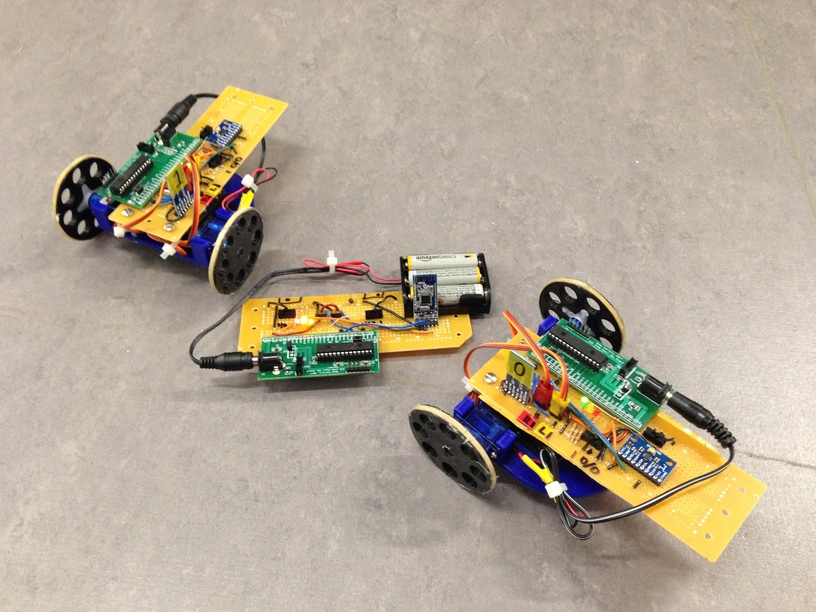
\includegraphics[width=0.8\textwidth]{full_system.jpg}
  \caption{Full system with 2 robots and the base station}
  \label{fig:robotsystem}
\end{figure}

\subsection{Design}

\subsubsection{Building the Robot}

The robots are made from 4 3D printed pieces: 2 wheels, the frame, and
the caster in the back.
Figure \ref{fig:robotchassis} shows the main components.
The servos, a 3 AA battery holder, and a perfboard containing all the circuitry are mounted directly to the frame.

\begin{figure}
  \centering
  \subfloat[Frame] {
    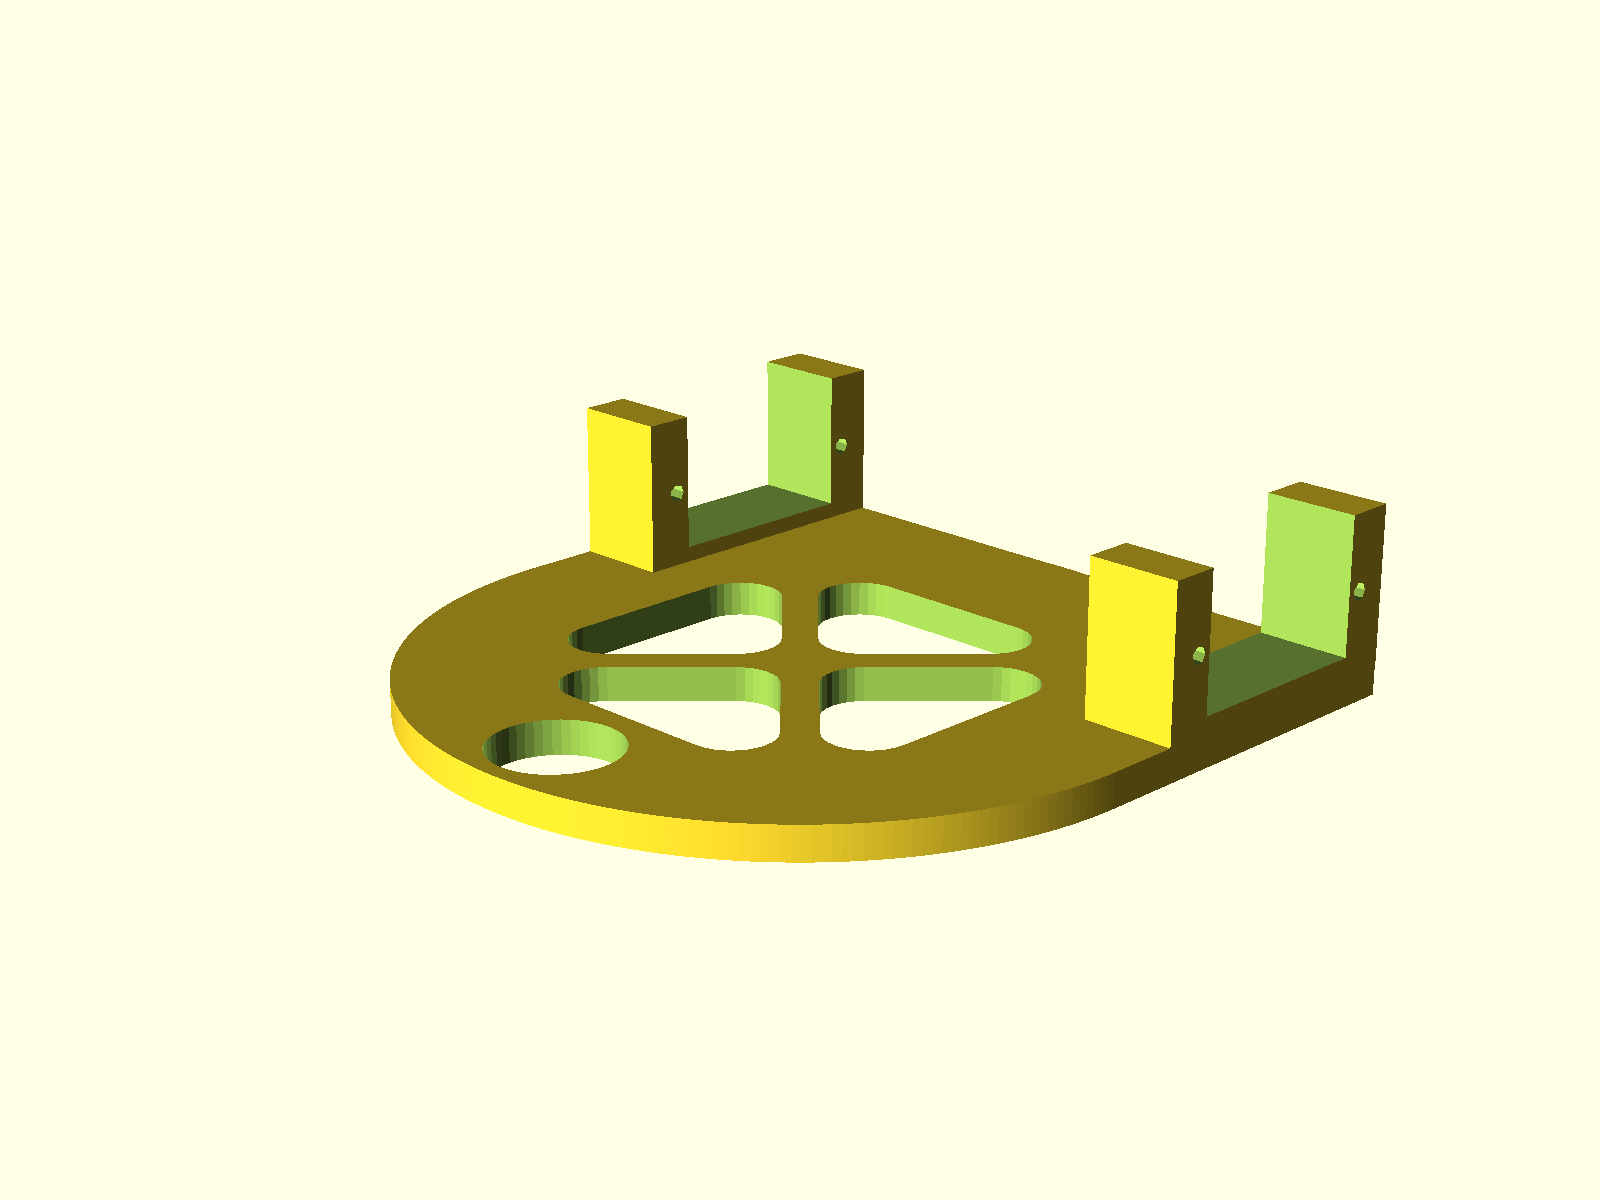
\includegraphics[width=0.4\textwidth,height=\textheight]{frame.png}
    \label{fig:robotfrane}
  }
  \subfloat[Wheel]{
    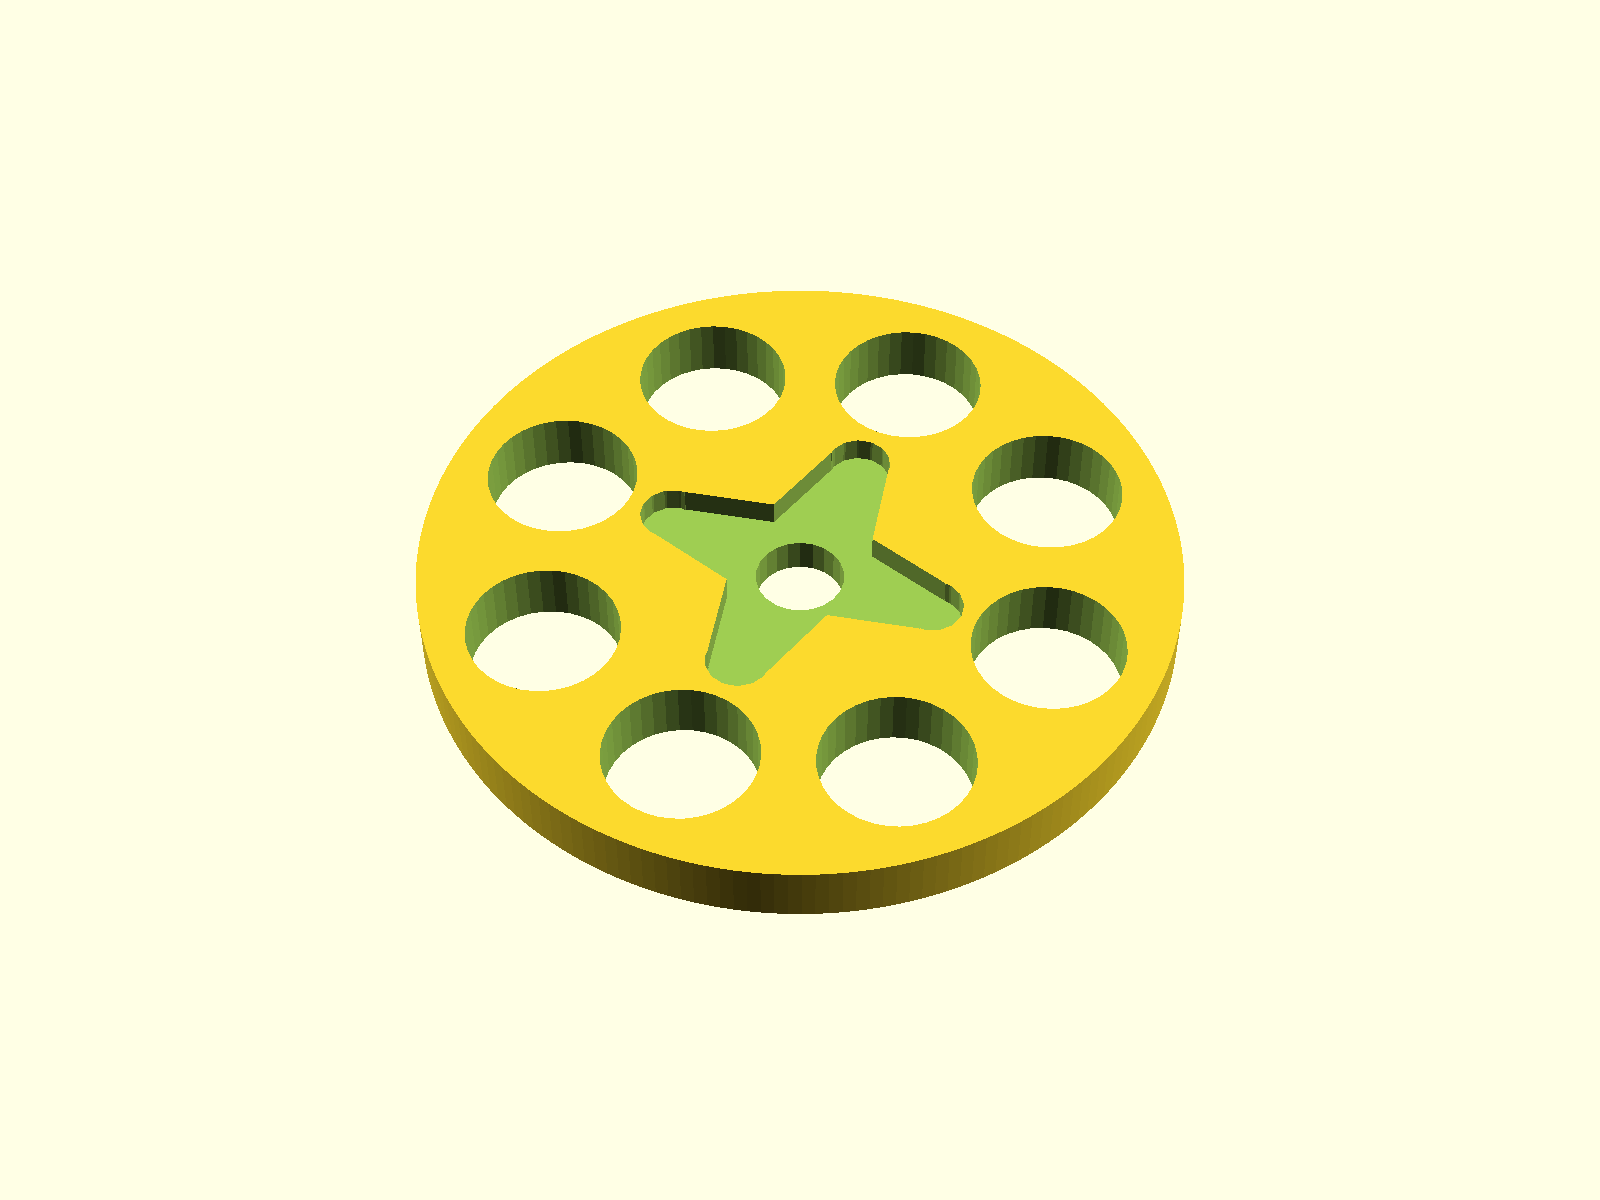
\includegraphics[width=0.4\textwidth,height=\textheight]{wheel.png}
    \label{fig:robotwheel}
  }
  \\
  \subfloat[Caster]{
    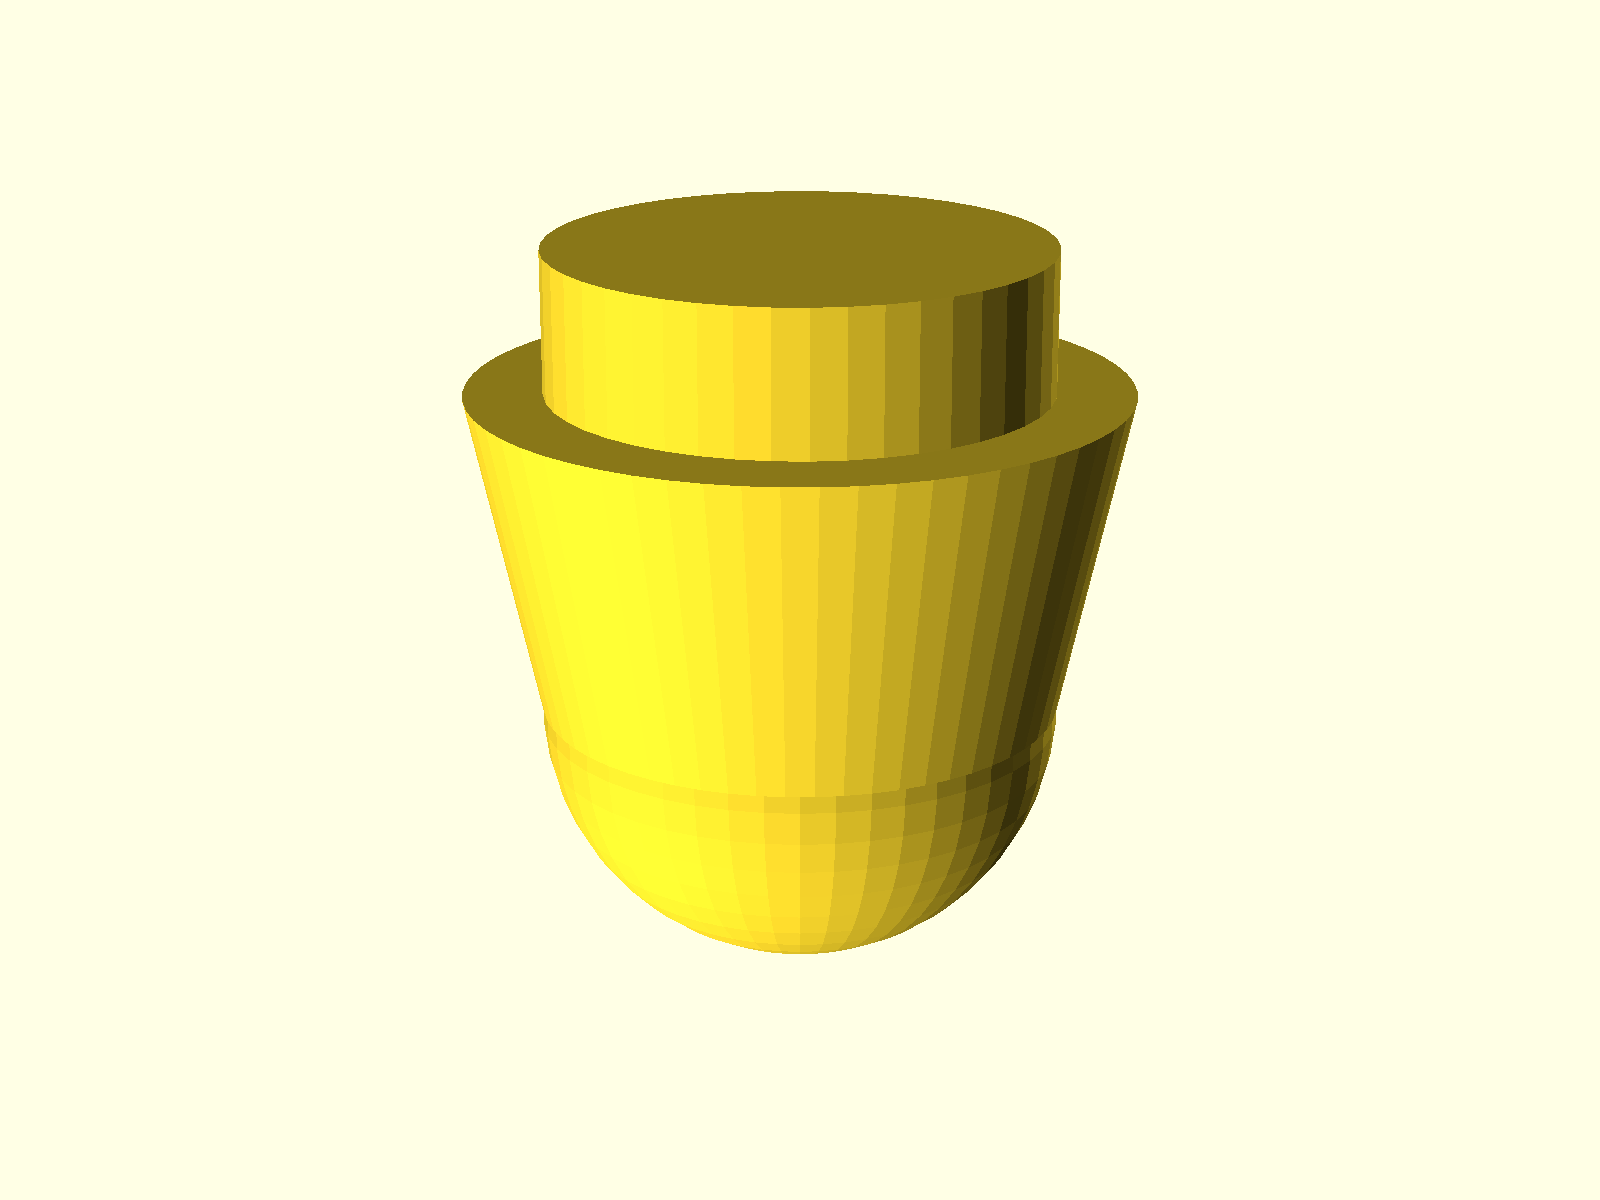
\includegraphics[width=0.4\textwidth,height=\textheight]{drag.png}
    \label{fig:robotcaster}
  }
  \caption{Components of robot chassis}
  \label{fig:robotchassis}
\end{figure}

The parts were printed in ABS using Maker Select 3D Printer v2 printers.
All parts were printed with a layer height of 0.3 mm, as there was no need for a smooth finish or high tolerances.
The parts were designed in OpenSCAD, and sliced with Cura.

% TODO: move around to be more top-down
Each robot consisted of 4 main components: a PIC32MC250F128B microcontroller, a MPU-9250 IMU with a 3 axis gryoscope, accelerometer, and magnetometer, a HM-10 BLE module with a Texas Instruments CC2541 chip, and two 9 gram FS90R micro continuous rotation servos.

The PIC32 and supporting circuity was on a small PCB (the ``Small Dev Board'' from ECE 4760 at Cornell University, the class during which we built this) shown in figure \ref{fig:schematic-sdb}. The rest of the components were assembled on solderable breadboard as shown in figure \ref{fig:schematic-robot}.

\begin{figure}
  \centering
  \subfloat[] {
    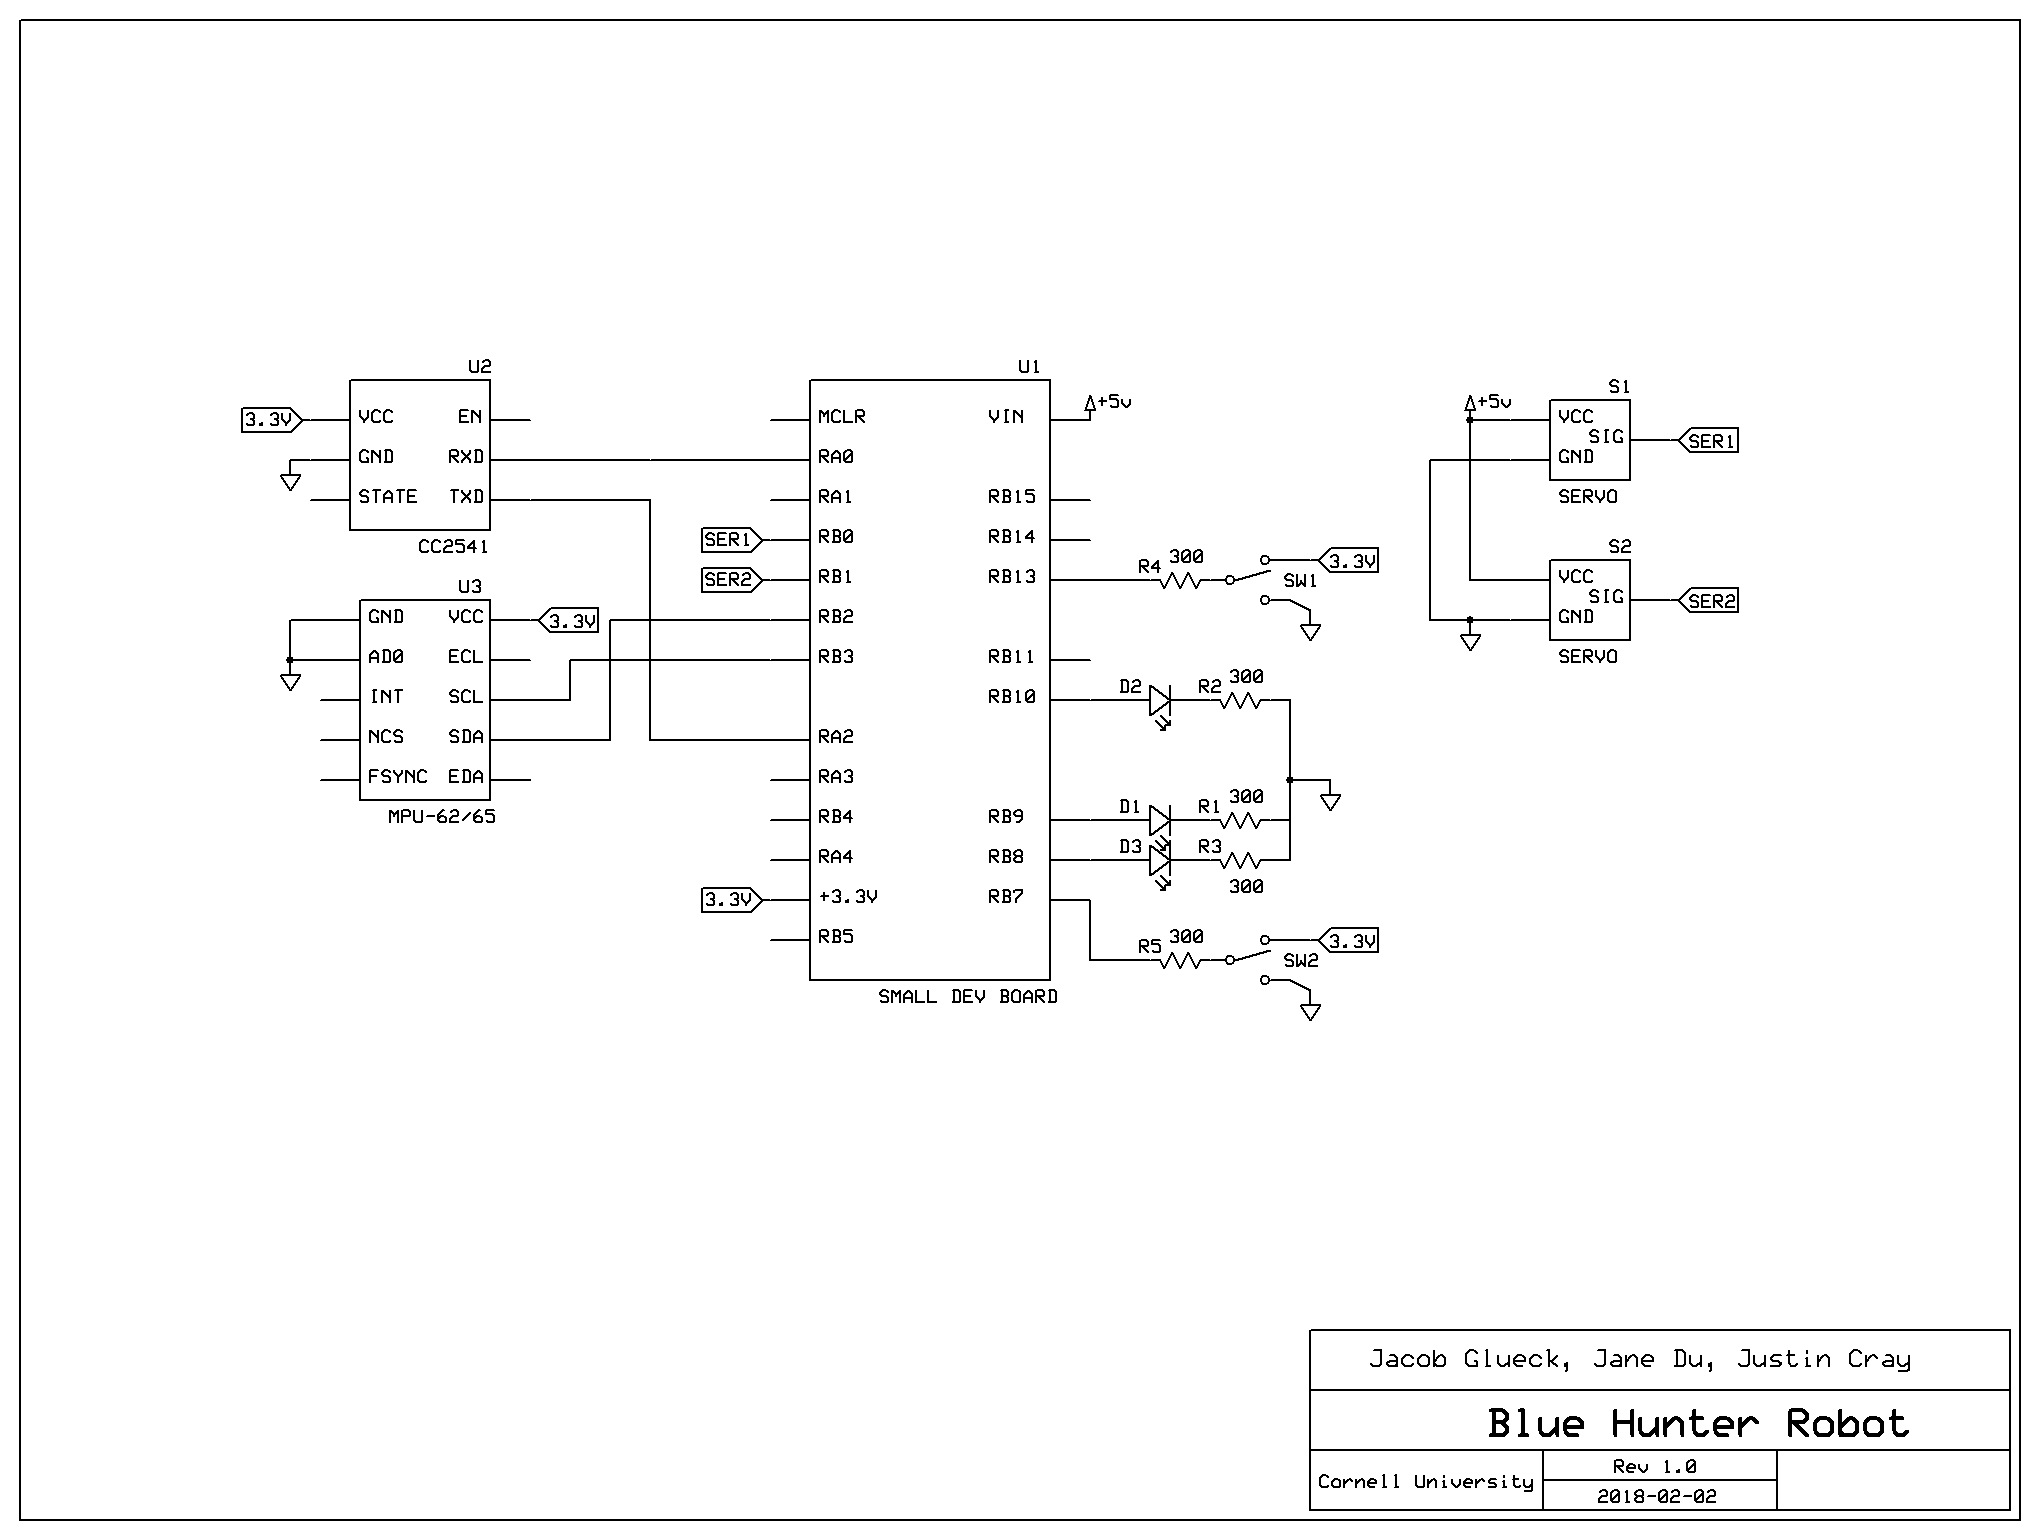
\includegraphics[width=0.9\textwidth]{bluehunters-robot.png}
    \label{fig:schematic-robot}
  }
  \\
  \subfloat[] {
    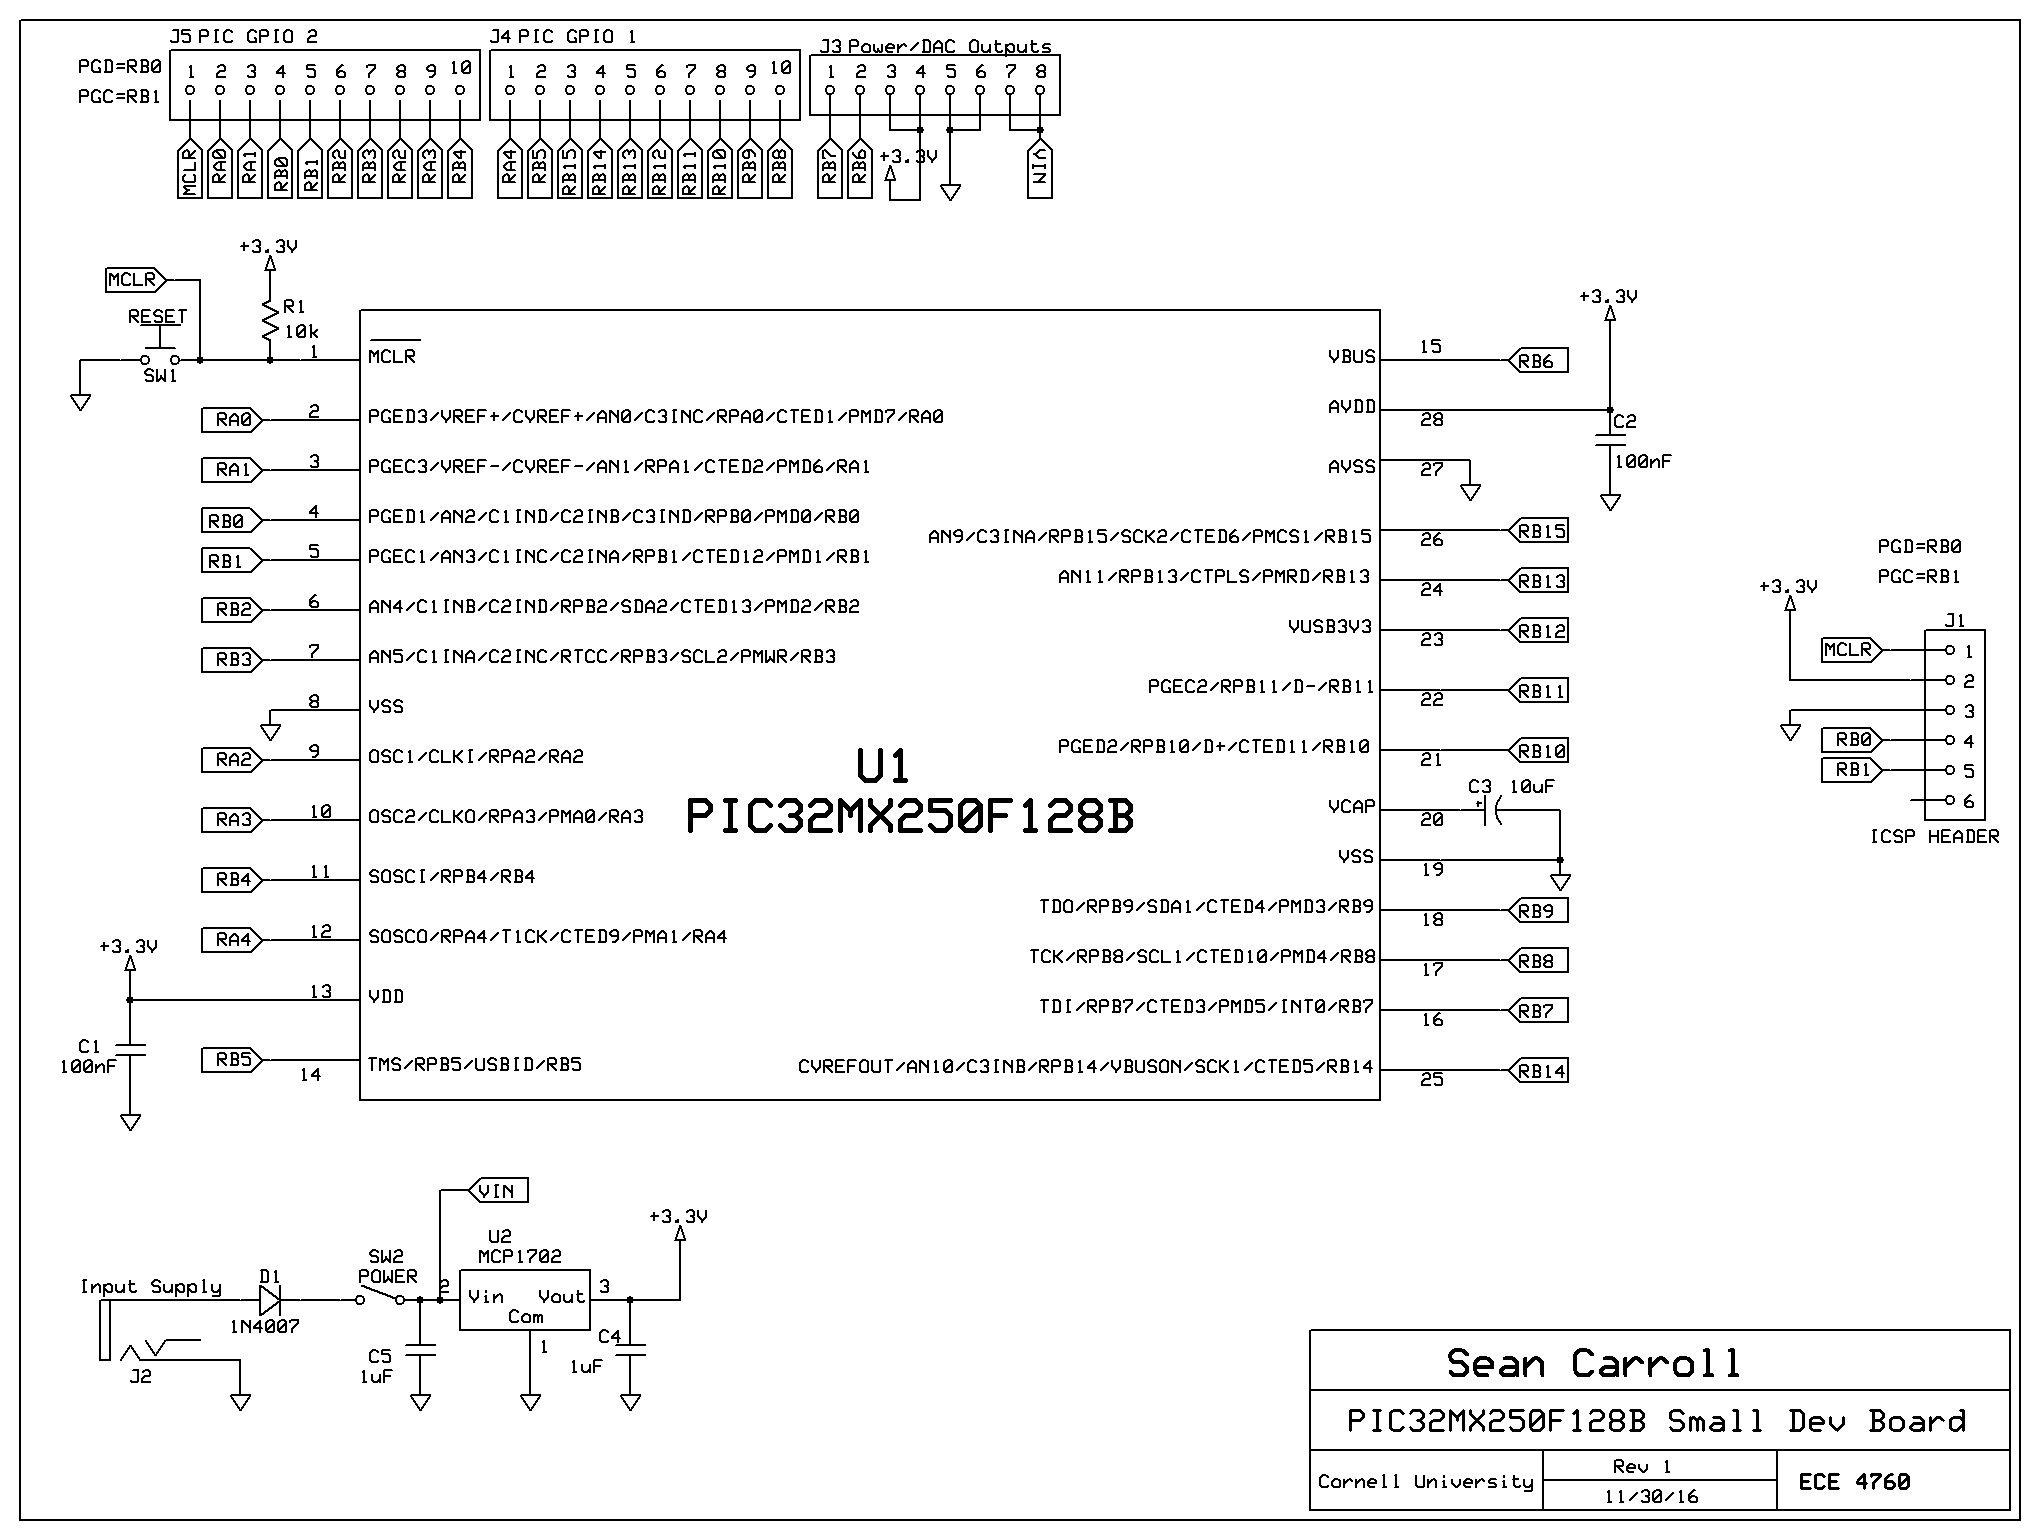
\includegraphics[width=0.9\textwidth]{bluehunters-sdb.png}
    \label{fig:schematic-sdb}
  }
  \caption{Schematic}
  \label{fig:schematic}
\end{figure}


For the drive system, we used FS90R servos.
These servos are continuous rotation servos with a stall torque of 1.5 kg-cm.
Like most servos, they are driven with PWM signals at 50 hertz (20 millisecond periods).
A duty cycle with about 1.5 milliseconds on is roughly neutral.
With the PIC32s running at 40 MHz, a prescaler of 32 and a maximum count of 25600 produces the required 50 hertz signal ($25600/\left(40\cdot 10^6 \frac{1}{\text{s}}/ 32 \right) = 0.02048 \text{ ms}$).
The PWM values (in timer counts) thus ranged from ranging from 1280 to 2560.


The robots were programmed in C, using MPLAB X IDE v4.0, the XC32 v1.4
compiler and the PIC 32 Legacy Peripheral Library (plib).
The full source code is available in online: \url{https://github.com/orangeturtle739/bluehunters/tree/master/ble.X}

\subsubsection{Signal Detection: Bluetooth Modules}

% Jnhuamao is the company which makes the HM-10 module, along with other Bluetooth modules. Their English website is: \url{http://www.jnhuamao.cn/bluetooth.asp?id=1}.

The HM-10 bluetooth modules we bought off Ebay were fakes: they were not made by Jnhuamao , and did not come with genuine Jnhuamao firmware.
However, they did have genuine TI CC2541 chips.
We realized they were fakes when they did not behave according to
the Jnhuamao data sheet at \cite{jnhuamaodatasheet},
with a PDF available at \cite{jnhuamaomit}, which may be out of date, but is easier to get.
Luckily, the hardware on the fake chips is the same as that of the genuine chips, minus an external crystal, and the genuine firmware checks for the presence of the crystal, and works even without
it. \cite{crystal}
As such, we reprogrammed the chips with the genuine firmware according
to an Arduino Fourm post \cite{crystal}:

\begin{enumerate}
\item
  We soldered wires to the programming pins on the breakout boards, and connected those pins to an Arduino Teensy 3.2.
  We chose a Teensy because it is 3.3 volts as opposed to 5, which would damage the 3.3 volt CC2541. The pins were connected as follows:

  \begin{longtable}[]{@{}lll@{}}
  \toprule
  Name & CC2541 Pin & Arduino Pin\tabularnewline
  \midrule
  \endhead
  \texttt{DEBUG\_CLOCK} & 7 & 5\tabularnewline
  \texttt{DEBUG\_DATA} & 8 & 6\tabularnewline
  \texttt{RESET\_N} & 11 & 4\tabularnewline
  \bottomrule
  \end{longtable}

  Figure \ref{fig:hm10} shows the layout of the HM-10 module.
  \begin{figure}
    \centering
    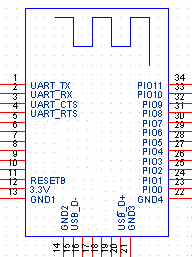
\includegraphics[width=0.3\textwidth]{hm10_pins.png}
    \caption{HM-10 module pin layout \cite{crystal}}
    \label{fig:hm10}
  \end{figure}

\item
  We uploaded the \texttt{CCLoader.ino} \cite{ccloader} sketch to the Arduino.
\item
  Finally, we ran (in a Windows virtual machine, due to the dubious origin of the software) \texttt{CCLoader.exe} \cite{ccloaderexe}.
  This program takes 3 arguments:

  \begin{Verbatim}[gobble=4]
    CCLoader.exe <COM Port> <Firmware.bin> 0
  \end{Verbatim}

  The firmware file came from the Arduino forum post. \footnote{The firmware file can be found here:  \url{http://forum.arduino.cc/index.php?action=dlattach;topic=393655.0;attach=183702}}
\end{enumerate}

After flashing genuine firmware onto the chip, the next step was to update the firmware to the latest version.
The firmware flashed onto the board was version 540, but Jnhuamao had (at the time we did this project) released version 603. \cite{jnhuamao603}
Based on their instructions \cite{jnhuamaoinstructions}, we flashed our chips:

\begin{enumerate}
\item
  Connect the HM-10 module to a computer using a 3.3 V FTDI to USB
  adapter. Then, use PUTTY to establish a serial session (9600 baud,
  8N1). Send the chip \texttt{AT}; if it is connected properly, it will
  respond with \texttt{OK}.
\item
  Send the chip \texttt{AT+SBLUP} to put it in firmware update mode. It
  will respond with \texttt{OK+SBLUP}. Terminate the PUTTY session.
\item
  Run the \texttt{HMSoft.exe} program distributed in the firmware update
  download. (Again in a Windows virtual machine, due to the dubious origin of the software.)
\item
  Select the proper port and firmware file using the software, and hit
  ``Load Image''. The software should handle the rest!
\item
  To make sure it worked, establish a serial connection again using
  PUTTY. Send \texttt{AT+VERS?} to query the chip for version
  information.
\end{enumerate}

The BLE module used UART, at 9600 baud 8N1. We used \texttt{UART1} on
the PIC for communicating with the BLE module, and used \texttt{UART2}
for communicating with the computer (for debugging).
We used the following commands to interact with the bluetooth chip:

% TODO: Tablify

\begin{itemize}
\item
  \texttt{AT+RESET}: resets the chip to ensure it is in a clean state
  before receiving other commands.
\item
  \texttt{AT+IBEA1}: enables the iBeacon functionality of the chip (sets
  it to 1; \texttt{AT+IBEA0} would disable it by setting it to 0). This
  allows the chip to be found with an RSSI scan. After setting the
  value, we query it with \texttt{AT+IBEA?} and send the result over the
  other serial port to a computer for debugging.
\item
  \texttt{AT+ROLE0} or \texttt{AT+ROLE1}: sets the role to either
  peripheral (0) or central (1). The base station is set to peripheral,
  and the 2 robots are set to central. Peripheral means the device will
  respond in inquiries from a central device. This allows it to be
  discovered during an RSSI scan. After setting the value, we query it
  with \texttt{AT+ROLE?} and send the result over the other serial port
  to a computer for debugging.
\item
  \texttt{AT+IMME0} or \texttt{AT+IMME1}: sets the work state of the
  device to either actively listening for Bluetooth signals (0), or only
  acting when it receives a serial command (1). Once again, the base
  station is set to 0: it needs to listen for signals and respond. The
  robots are set to 1, as the chips need to initiate scan requests when
  they receive the command over serial. After setting the value, we
  query it with \texttt{AT+IMME?} and send the result over the other
  serial port to a computer for debugging.
\item
  \texttt{AT+NAME\%s}: sets the name of the chip (which is visible when
  scanning) to \texttt{\%s} (For example, \texttt{AT+NAMEPIRATE} names
  the chip \texttt{PIRATE}). We give all the chips unique names to make
  debugging easier. After setting the value, we query it with
  \texttt{AT+NAME?} and send the result over the other serial port to a
  computer for debugging.
\item
  \texttt{AT+SHOW3}: configures the device to advertise both its name
  and RSSI when scanning.
\item
  \texttt{AT+ADDR?}: queries the device for its hardware address. We
  recorded the hardware device of each chip, as when doing RSSI scans,
  the results are reported by hardware address.
\item
  \texttt{AT+DISI?}: performed only on the robots, causing a discovery
  scan. The result of the scan is a series of lines of the form:

\begin{verbatim}
OK+DISC:00000000:00000000000000000000000000000000:
  0000000000:6832A3801EBE:-080
\end{verbatim}

  The second to last token, \texttt{6832A3801EBE}, is the hardware
  address of the discovered device, and the last token, \texttt{-080},
  is the measured RSSI. The chip will transmit a line for each device it
  finds (``line'' is a misnomer as it does not separate them with any
  characters), followed by \texttt{OK+DISCE}.
\end{itemize}

One interesting thing to note about the chip is that commands do not have to end with newlines or carriage returns.
However, if sent, the chip will ignore them.

\subsubsection{Navigation}

After measuring the proximity to the beacon, the robots would need to move towards it. The robot made use of the magnetometer (compass) inside the IMU to orient itself, and the gradient descent algorithm to decide the direction of its next movement.

For the IMU, we used the QFN MPU-9250 \cite{mpu9250datasheet} \cite{mpu9250regmap} module. It has 2 dies: one is the AK8963 3-axis magnetometer \cite{ak8963cdatasheet}, and the other contains the 3-axis gyroscope and 3-axis accelerometer, which were not used in this project.

The microcontroller communicates with the IMU via I2C, and the compass is connected to the rest of the MPU module via an auxiliary I2C bus. For communication between the microcontroller and the AK8963's main die, we based our work off of basic I2C functions from another ECE 4760 project, the Self-Balancing Robot \cite{selfbalancingrobot}. In particular, their \texttt{i2c\_helper.h} was very helpful.

For communication with the actual magnetometer, we needed to configure the IMU to set the compass must as a slave on the I2C bus. For this, it was necessary to enable pass-through mode on the IMU during its configuration.

The AK8963 has several modes of operation, and the chip must be set to power-down mode before switching to other modes.
We read compass values with single measurement mode, as in figure \ref{fig:imu_single_measurement}.

A single compass read involves setting the compass to single measurement mode in 14 bit resolution, reading the 6 data registers (X low, X high, Y low, Y high, Z low, Z high), reading the Status 2 register to check for magnetic sensor overflow (without reading this register, the read is not considered complete and further reads will fail), and finally waiting to ensure that the IMU is not read too frequently, in which case it will not have enough time to take measurements.

\begin{figure}
  \centering
  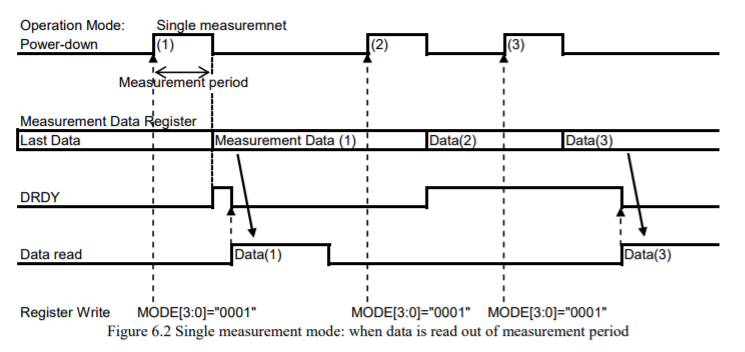
\includegraphics[width=0.9\textwidth]{imu_single_measurement.png}
  \caption{IMU single measurement mode}
  \label{fig:imu_single_measurement}
\end{figure}

In order to calibrate the compass, the robots spun in place when powered
on.
They recorded the maximum and minimum values for each axes, and used
that data to scale and center the magnetometer readings.

The algorithm for deciding what path to follow is a basic version of
gradient descent. Figure \ref{fig:graddesc} shows 2 versions of the gradient descent algorithm.

\begin{figure}
  \centering
  \subfloat[Simple gradient descent]{
    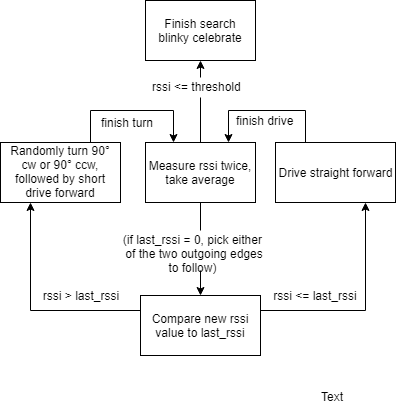
\includegraphics[width=0.4\textwidth]{grad_desc.png}
    \label{fig:simplegrad}
  }
  \subfloat[Compensating gradient descent]{
      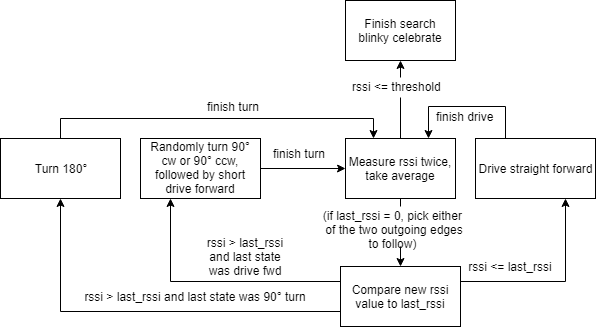
\includegraphics[width=0.5\textwidth]{turn_correction.png}
    \label{fig:compensatinggrad}
  }
  \caption{2 gradient descent algorithms. The initial state is \emph{measure RSSI twice, take average}.}
  \label{fig:graddesc}
\end{figure}

The purpose of the compensating algorithm (figure \ref{fig:compensatinggrad}) was to allow the robots to recover faster after taking a wrong turn: if a robot just just moved forward and detected a weaker signal, turned, and still detected a weaker signal, then it must have turned the wrong way, so it does a 180.
However, it did not prove any more accurate than randomized gradient descent, largely due to noisy RSSI readings.
As such, we used the simplified version.

\subsection{Results}

In most cases, at least 1 of the 2 robots successfully made it to the
base station. However, it was not as reliable as we initially hoped. One
of the main reasons for this was the noise in RSSI measurements.

We expected that RSSI would vary with distance according to equation \ref{eq:rssi}:
\begin{equation} \label{eq:rssi}
  \text{RSSI} = A - 10 n \log(d),
\end{equation}
where $A$ and $n$ are RF propagation parameters in dBm, $d$ is distance in meters, and RSSI is the measured RSSI in dBm. \cite{5415423}
We experimented with RSSI measurements to determine how well they worked by taking 2 Bluetooth modules, and measuring the RSSI while moving them apart.
One remained stationary on the floor and the other was moved away from it 1 foot at a time.
At each point, we took 3 RSSI measurements and averaged them. Figure \ref{fig:rssiplot} shows the results (the original data is in table \ref{table:rssidata}).

\begin{figure}
  \centering
  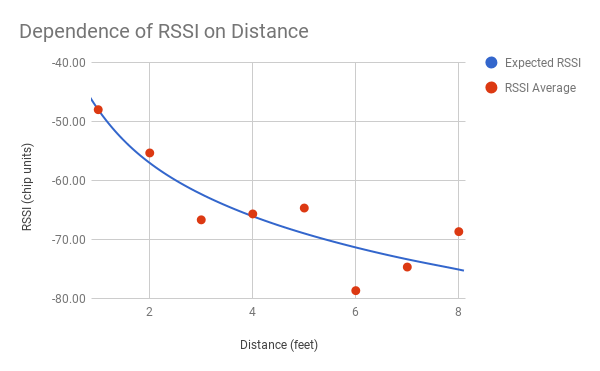
\includegraphics[width=0.9\textwidth]{rssi-chart.png}
  \caption{Plot showing bluetooth RSSI as a function of distance}
  \label{fig:rssiplot}
\end{figure}

\begin{table}
  \centering
  \begin{tabular}[]{@{}llllll@{}}
  \toprule
  Distance (feet) & RSSI A & RSSI B & RSSI C & RSSI Average & Expected
  RSSI \\
  \midrule
  1 & -48 & -48 & -48 & -48.00 & -48.00 \\
  2 & -56 & -58 & -52 & -55.33 & -57.03 \\
  3 & -66 & -66 & -68 & -66.67 & -62.31 \\
  4 & -64 & -68 & -65 & -65.67 & -66.06 \\
  5 & -60 & -70 & -64 & -64.67 & -68.97 \\
  6 & -80 & -80 & -76 & -78.67 & -71.34 \\
  7 & -80 & -79 & -65 & -74.67 & -73.35 \\
  8 & -68 & -66 & -72 & -68.67 & -75.09 \\
  \bottomrule
  \end{tabular}
  \caption{RSSI and distance data}
  \label{table:rssidata}
\end{table}

\begin{table}[]
\centering
\ra{1.3}
\caption{Convergence performance of the robots}
\label{table:convergence}
\begin{tabular}{@{}lllllll@{}}
\toprule
\multirow{2}{*}{Trial} & \multicolumn{3}{c}{Robot 0}       & \multicolumn{3}{c}{Robot 1}      \\ \cmidrule(l){2-4} \cmidrule(l){5-7}
                       & Time (s)  & Distance (cm) & Start & Time (s) & Distance (cm) & Start \\ \midrule
1                      & 213       & 53            & South & 94       & 22            & North \\
2                      & \emph{Collision} & 420           & South & 153      & 36            & North \\
3                      & 308       & 19            & South & 105      & 36            & North \\
4                      & \emph{Collision} & 340           & South & 80       & 20            & North \\
5                      & \emph{Collision} & 240           & South & 92       & 30            & North \\
6                      & 179       & 46            & North & 117      & 20            & South \\
7                      & 56        & 45            & North & 162      & 24            & South \\
8                      & 59        & 27            & North & 197      & 26            & South \\
9                      & 59        & 19            & North & 79       & 30            & South \\
10                     & \emph{Collision} & 231           & North & 67       & 23            & South \\ \bottomrule
\end{tabular}
\end{table}

While the chip reported RSSI in units proportional to dBm, and we
measured distances in feet, not meters, we could still use the above
formula without worrying about unit conversions. The constants $A$ and
$n$, provided we determined them empirically based on the data, would
encode the conversions. As such, we fit the data using the above formula
with $A=-48$ and $n=3$, resulting in the blue curve above. While the
general shape of the curve matches, there is significant noise in the
averaged RSSI data. Furthermore, when we tried to reproduce the
measurements, we could not do so precisely -- it seemed to even depend
on where our feet where!

Despite how noisy the RSSI measurements where, the robots were still
able to perform a reasonably accurate gradient descent. In most cases,
at least one of the 2 robots would find the beacon in a matter of
minutes.

\subsection{Conclusions}

This project was an interesting exploration into short-range distance
determination using Bluetooth, a generally unconventional approach.
We knew that Bluetooth RSSI would be noisy, mostly due to multipath interference and the presence of multiple transmitters in testing environments.
The robots worked reliably when they stayed within roughly 1 meter of the beacon.
After this, they entered the land of shallow gradients:
the signal strength from the beacon (already noisy) would not change very
much, and often only due to noise.
They normally could never recover from this.



There are many potential avenues for improvements or further
development.

Firstly, \emph{Communication between the two robots}: while Bluetooth may not offer good distance measurement via RSSI, it can be used for reliable  communication between modules.
It would be straightforward for one hunting robot to inform the other whether it believes it is approaching the beacon or not.
In the simplest case, a robot that is approaching, or already at, the beacon can provide a second point of reference for a currently hunting robot.

Also, \emph{More complete usage of IMU}: additional usage of the accelerometer and gyroscope, coupled with feedback from the servos, would allow the robots to maintain a dead-reckoning position estimate.
This, paired with inter-swarm communication, would make for a much more sophisticated and likely much more efficient system.
(Of course, this does not resolve the shallow gradients problem -- but it would allow the approach to the beacon to be much faster.)

\bibliography{references}{}
\bibliographystyle{ieeetr}


\begin{appendices}
  \section{Bill Of Materials}
  This project was done with a \$150 budget in mind. Costs for parts labeled ``Lab rental'' were borrowed from the department of Electrical and Computer Engineering at Cornell University, but can also be found at vendors like Digikey, Adafruit, and Amazon.

  \begin{centering}
  \tiny
  \begin{longtable}[]{@{}lllllll@{}}
  \toprule
  \begin{minipage}[b]{0.15\columnwidth}\raggedright
  Name\strut
  \end{minipage} & \begin{minipage}[b]{0.15\columnwidth}\raggedright
  Manufacturer Part Number\strut
  \end{minipage} & \begin{minipage}[b]{0.10\columnwidth}\raggedright
  Vendor\strut
  \end{minipage} & \begin{minipage}[b]{0.17\columnwidth}\raggedright
  Vendor Part Number\strut
  \end{minipage} & \begin{minipage}[b]{0.11\columnwidth}\raggedright
  Quantity\strut
  \end{minipage} & \begin{minipage}[b]{0.06\columnwidth}\raggedright
  Unit Cost\strut
  \end{minipage} & \begin{minipage}[b]{0.07\columnwidth}\raggedright
  Total Cost\strut
  \end{minipage}\tabularnewline
  \midrule
  \endhead
  \begin{minipage}[t]{0.15\columnwidth}\raggedright
  BLE 4.0 Module (TI CC2541)\strut
  \end{minipage} & \begin{minipage}[t]{0.15\columnwidth}\raggedright
  HM-10\strut
  \end{minipage} & \begin{minipage}[t]{0.10\columnwidth}\raggedright
  \href{https://www.ebay.com/itm/AT-09-BLE-Bluetooth-4-0-Uart-Transceiver-Module-CC2541-Central-Switching-HM-10/142425748901?ssPageName=STRK\%3AMEBIDX\%3AIT\&_trksid=p2057872.m2749.l2649}{Ebay}\strut
  \end{minipage} & \begin{minipage}[t]{0.17\columnwidth}\raggedright
  142425748901\strut
  \end{minipage} & \begin{minipage}[t]{0.11\columnwidth}\raggedright
  3\strut
  \end{minipage} & \begin{minipage}[t]{0.06\columnwidth}\raggedright
  \$3.99\strut
  \end{minipage} & \begin{minipage}[t]{0.07\columnwidth}\raggedright
  \$11.97\strut
  \end{minipage}\tabularnewline
  \begin{minipage}[t]{0.15\columnwidth}\raggedright
  FEETECH FS90R (pack of 2) Continuous Rotation Robotic Servo\strut
  \end{minipage} & \begin{minipage}[t]{0.15\columnwidth}\raggedright
  FS90R\strut
  \end{minipage} & \begin{minipage}[t]{0.10\columnwidth}\raggedright
  \href{https://www.amazon.com/gp/product/B074BFQC3Q/ref=oh_aui_detailpage_o06_s00?ie=UTF8\&psc=1}{Amazon}\strut
  \end{minipage} & \begin{minipage}[t]{0.17\columnwidth}\raggedright
  B074BFQC3Q\strut
  \end{minipage} & \begin{minipage}[t]{0.11\columnwidth}\raggedright
  2\strut
  \end{minipage} & \begin{minipage}[t]{0.06\columnwidth}\raggedright
  \$12.39\strut
  \end{minipage} & \begin{minipage}[t]{0.07\columnwidth}\raggedright
  \$24.78\strut
  \end{minipage}\tabularnewline
  \begin{minipage}[t]{0.15\columnwidth}\raggedright
  HiLetgo 9-Axis 9 DOF 16 Bit Gyroscope Acceleration Magnetic Sensor\strut
  \end{minipage} & \begin{minipage}[t]{0.15\columnwidth}\raggedright
  MPU-9250\strut
  \end{minipage} & \begin{minipage}[t]{0.10\columnwidth}\raggedright
  \href{https://www.amazon.com/HiLetgo-Gyroscope-Acceleration-Accelerator-Magnetometer/dp/B01I1J0Z7Y/ref=redir_mobile_desktop?_encoding=UTF8\&dpID=51nl2fcMh6L\&dpPl=1\&keywords=mpu\%209250\&pi=AC_SX236_SY340_QL65\&qid=1512564044\&ref=plSrch\&ref_=mp_s_a_1_3\&sr=8-3}{Amazon}\strut
  \end{minipage} & \begin{minipage}[t]{0.17\columnwidth}\raggedright
  B01I1J0Z7Y\strut
  \end{minipage} & \begin{minipage}[t]{0.11\columnwidth}\raggedright
  2\strut
  \end{minipage} & \begin{minipage}[t]{0.06\columnwidth}\raggedright
  \$8.49\strut
  \end{minipage} & \begin{minipage}[t]{0.07\columnwidth}\raggedright
  \$16.98\strut
  \end{minipage}\tabularnewline
  \begin{minipage}[t]{0.15\columnwidth}\raggedright
  Small board\strut
  \end{minipage} & \begin{minipage}[t]{0.15\columnwidth}\raggedright
  --\strut
  \end{minipage} & \begin{minipage}[t]{0.10\columnwidth}\raggedright
  Lab rental\strut
  \end{minipage} & \begin{minipage}[t]{0.17\columnwidth}\raggedright
  --\strut
  \end{minipage} & \begin{minipage}[t]{0.11\columnwidth}\raggedright
  3\strut
  \end{minipage} & \begin{minipage}[t]{0.06\columnwidth}\raggedright
  \$5.00\strut
  \end{minipage} & \begin{minipage}[t]{0.07\columnwidth}\raggedright
  \$15.00\strut
  \end{minipage}\tabularnewline
  \begin{minipage}[t]{0.15\columnwidth}\raggedright
  PIC32MX250F128B\strut
  \end{minipage} & \begin{minipage}[t]{0.15\columnwidth}\raggedright
  PIC32MX250F128B\strut
  \end{minipage} & \begin{minipage}[t]{0.10\columnwidth}\raggedright
  Lab rental\strut
  \end{minipage} & \begin{minipage}[t]{0.17\columnwidth}\raggedright
  --\strut
  \end{minipage} & \begin{minipage}[t]{0.11\columnwidth}\raggedright
  3\strut
  \end{minipage} & \begin{minipage}[t]{0.06\columnwidth}\raggedright
  \$5.00\strut
  \end{minipage} & \begin{minipage}[t]{0.07\columnwidth}\raggedright
  \$15.00\strut
  \end{minipage}\tabularnewline
  \begin{minipage}[t]{0.15\columnwidth}\raggedright
  6-inch Protoboard\strut
  \end{minipage} & \begin{minipage}[t]{0.15\columnwidth}\raggedright
  --\strut
  \end{minipage} & \begin{minipage}[t]{0.10\columnwidth}\raggedright
  Lab rental\strut
  \end{minipage} & \begin{minipage}[t]{0.17\columnwidth}\raggedright
  --\strut
  \end{minipage} & \begin{minipage}[t]{0.11\columnwidth}\raggedright
  3\strut
  \end{minipage} & \begin{minipage}[t]{0.06\columnwidth}\raggedright
  \$2.50\strut
  \end{minipage} & \begin{minipage}[t]{0.07\columnwidth}\raggedright
  \$7.50\strut
  \end{minipage}\tabularnewline
  \begin{minipage}[t]{0.15\columnwidth}\raggedright
  Male header pins\strut
  \end{minipage} & \begin{minipage}[t]{0.15\columnwidth}\raggedright
  --\strut
  \end{minipage} & \begin{minipage}[t]{0.10\columnwidth}\raggedright
  Lab\strut
  \end{minipage} & \begin{minipage}[t]{0.17\columnwidth}\raggedright
  --\strut
  \end{minipage} & \begin{minipage}[t]{0.11\columnwidth}\raggedright
  129\strut
  \end{minipage} & \begin{minipage}[t]{0.06\columnwidth}\raggedright
  \$0.05\strut
  \end{minipage} & \begin{minipage}[t]{0.07\columnwidth}\raggedright
  \$6.45\strut
  \end{minipage}\tabularnewline
  \bottomrule
  \end{longtable}
  \end{centering}

  \textbf{Total:} \$97.68
\end{appendices}

\end{document}
